\documentclass[12pt]{article}

\author{Pablo Vargas Bermúdez}

\usepackage{minted}
\usepackage[margin=3cm]{geometry}
\usepackage{pdfpages}
\usepackage{graphicx}

\begin{document}
\pagestyle{empty}

% \inlcudepdf[pages=-]{Portada}

\section*{Planteamiento}

Cree un programa que mediante un interfaz Gráfica permita a
seleccionar una Carrera de las que imparte el ITL asi como el turno.

Utiliza el componente JRadioButton y ButtonGroup para que se pueda
seleccionar solamente una carrera y un turno.

\section*{Código}

\subsection*{Clase de Gui}
\inputminted{Java}{Carreras.java}
\subsection*{Clase de prueba}
\inputminted{Java}{Prueba.java}

\section*{Ejecución}

\begin{figure}[ht]
  \centering
  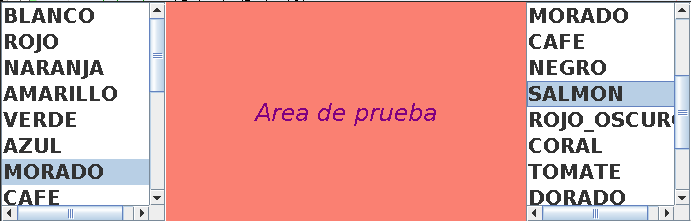
\includegraphics[width=\textwidth]{figures/run1.png}
  \caption{Primera prueba}
\end{figure}

\begin{figure}[ht]
  \centering
  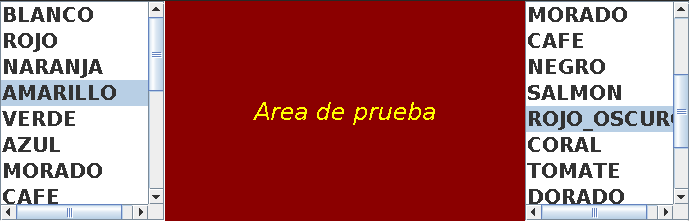
\includegraphics[width=\textwidth]{figures/run2.png}
  \caption{Segunda prueba}
\end{figure}

\end{document}
